\chapter{Federated Learning and Machine Learning} \label{chap:federated-learning}
\section{Introduction to machine learning}
One of the central topics of this document is Federated Learning, however, before introducing it in depth, we
must first introduce the subject to which it belongs: machine learning.
What is machine learning and what is its underlying problem? Machine
learning is the discipline which seeks to answer the following
question: \emph{"how can a computer improve based on experience?"}.

There are three main branches of machine learning:
\begin{enumerate}
  \item Supervised learning
  \item Unsupervised learning
  \item Reinforcement learning
\end{enumerate}

Federated learning was originally born as a supervised learning technique, however recent work has been done to bring
ito unsupervised \cite{UnsupervisedFL} and reinforcement learning \cite{ReinforcementFL}.
A short summary of all three learning methods is the following:
\begin{itemize}
  \item Supervised learning about generalizing a dataset of examples to produce a general rule that can be
    applied to new examples.
  \item Unsupervised learning is about finding patterns and relationship between examples of the dataset.
  \item Reinforcement Learning studies how well a machine is able to adapt to a dynamic environmnet based on
    reward and penalties.
    When the machine does 'well' it receives a reward, otherwise it recieves a penalty.
\end{itemize}
For the sake of this document we will only cover supervised learning in a little more depth.

If the reader is interested in diving deeper into the topic of machine learning and gain a more thorough
understanding of the techniques adopted and discussed here we suggest to take a look at \cite{MLBook}.

\section{Supervised Learning}\label{sec:supervised-learning}

Supervised Learning is the task of turning a dataset of input-output
pairs into a general rule that should be able to produce the correct
output even for inputs not necessarily seen in the original dataset.

The inputs and outputs are usually denoted respectively with the
symbols \(x\) and \(y\).
Therefore, our rule will be the function \(f\) for which we would
like \(y = f(x)\).

\subsection{Dataset}
A dataset is a collection of unordered \textit{observations} of
input/output pairs.
Each input is composed of a set of \textit{features} or
\textit{attributes}, while the outputs contain \textit{labels}
or \textit{targets}.
Generally the inputs contain many features while the outputs are
scalar values and every input and output of the dataset has the same
features and labels,
however this needn't hold true.

Suppose that the examples of the dataset have \(n\) features and that
the number of examples in the dataset is \(m\). The dataset can be
represented as a pair of matrices \(X\) and \(Y\) where \(X\) is \(m
\times n\) and \(Y\) is \(m \times 1\). The convention is to
represent vectors as columns, so the rows of \(X\) will be the
transposed input vectors.

The features and the label can be categorized into:
\begin{itemize}
  \item \textbf{Categorical}: For example relationship status
    (married, single, divorced, \dots)
  \item \textbf{Real-valued}: For example weight or height
  \item \textbf{Binary}: Boolean values (true/false, 0/1, yes/no, \dots)
\end{itemize}

As already stated, the goal is to produce a rule that generalizes
well to the examples so that it can work on yet-unseen ones. This rule is called a
\textit{classifier} if the label is categorical, whereas it is called
a \textit{regressor} if it is real-valued.

\subsection{Assumptions of supervised learning} \label{sec:assumptions-supervised-learning}
We assume that the input/output examples contained in the dataset are
chosen at random from
the target population (the dataset is technically a \textit{sample}
of the population).
Another assumption we make is that examples of the dataset are
independent from each other and belong to the same
distribution, which is called \textbf{IID Assumption} (independent
and identically distributed).
This assumption is quite strong and will also be discuted later in
\ref{sec:vanilla-fl}

\subsection{Common Approach to Supervised Learning}
A common approach to supervised learning is the so-called
\textit{discriminative approach}, which involves the following steps:
\begin{enumerate}
  \item Define an error measurement.
  \item Define a hypothesis space, which is the set of all the rules
    that we can accept.
  \item Pick the rule inside the hypothesis space for which the error
    on the training set is minimized.
\end{enumerate}

This approach has its own pitfalls: we might choose a rule that
matches perfectly the training set but does not generalize well. This
is called \textit{overfitting} and can be seen in \ref{fig:overfitting}
polynomial below. The opposite of this is called
\textit{underfitting}.
\begin{figure}[h!]
  \centering
  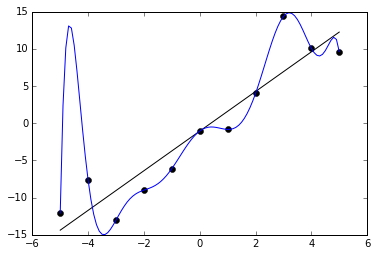
\includegraphics[width=0.8\textwidth]{figures/ml/overfitted_data.png}
  \caption[Overfitted data visualization]{Overfitted data visualization. One can see that the
    polynomial fits perfectly the training set but does likely not
  generalize well.}
  \begin{minipage}{0.8\textwidth}
    \begin{center}
      \footnotesize
      Source:
      \href{https://commons.wikimedia.org/wiki/File:Overfitted_Data.png}{Wikimedia
      Commons}, licensed under CC BY-SA 4.0.
    \end{center}

  \end{minipage}
  \label{fig:overfitting}
\end{figure}
To mitigate this problem, we split the data into the \textbf{training
set} and the \textbf{testing set}. The former is used for training
our model and creating our rule, whereas the latter is used solely
for testing our rule.

\clearpage

\section{Gradient Descent Algorithm} \label{sec:gradient-descent}
Consider a function \( f : \mathbb{R}^{n} \to \mathbb{R} \) at least
of class \(C^{1}\), that we want to minimize.
In case of simple functions, it is possible to accomplish this task with precise mathematical methods.
As an example consider the function \( f(x) = x^{2} \).
The minimum can be precisely found by studying its first and second derivatives.

However this is not always possible or practical to do.
This is often the case in machine learning where the loss functions we want to minimize are very complex.

That's why optimization is usually performed via iterative methods, the most common of which is the gradient
descent algorithm.
There are multiple variations, but the general concept is to start somewhere in the parameter space (e.g
$\mathbb R^n$), keep \textit{"moving"} towards the direction of fastest decrease and stop once a satisfactory
point of minimum is near.

The direction of fastest decrease of a differentiable function is given by the negative gradient of the function.
This is true because by definition:
\[
  \frac{\partial f}{\partial v}(\vec x) = \vec \nabla f(\vec x) \cdot \vec v = \| \vec \nabla f(\boldsymbol
  x)\| \cdot \|\vec v\| \cos \theta
\]
Thus the vector which minimizes the directional derivative is the one in the opposite direction of the
gradient (i.e. for which $\theta = -180^{\circ}$).

The classic gradient descent algorithm works as follows:

\begin{algorithmic}[1]
  \State Pick a starting vector \( \vec{w} \) and a step size \( \eta \).

  \While{not convergence}
  \State \( g \gets \nabla f(\vec{w}) \)
  \State \( \vec{w} \gets \vec{w} - \eta g \)
  \EndWhile
\end{algorithmic}

If the step size is too big, the minimum might be skipped; if it is
too small, the algorithm might take a long time to converge.
Usually, the step size is chosen adaptively.

\textbf{When is convergence reached?}
\begin{itemize}
  \item The gradient is near to zero.
  \item The objective function is not changing by more than a certain
    threshold between steps.
\end{itemize}

\subsection{Variations}
Gradient descent techniques are a field of ongoing research thus it would not be feasible to cover all the variations.
However we consider the case where the function \( f \) is a sum of functions \( f(\vec{w}) =
\sum_{i=1}^{m} f_{i}(\vec{w}) \).
In this case there are two canonical variations of the gradient descent algorithm: the batch and the
stochastic gradient descent.

\subsubsection*{Batch Gradient Descent} \label{sec:batch-gradient-descent}
The batch gradient descent is simply the same gradient descent algorithm described above with the difference that
the gradient $\nabla f(\vec{w})$ is calculated via linear superposision of the gradients of the single
functions $f_{i}(\vec{w})$:
\[
  \nabla f(\vec{w}) = \sum_{i=1}^{m} \nabla f_{i}(\vec{w})
\]
So the algorithm becomes:

\begin{algorithmic}[1]
  \While{not minimum}
  \State \( g = 0 \)
  \For{\( i = 1 \) to \( m \)}
  \State \( g \gets g + \nabla f_i(\vec{w}) \)
  \EndFor
  \State \( \vec{w} -= \eta g \)
  \EndWhile
\end{algorithmic}

This kind of algorithm is an \textit{offline}, as \( \vec{w}
\) is changed only at the end.

\subsubsection*{Stochastic Gradient Descent} \label{sec:stochastic-gradient-descent}
The stochastic variation of the gradient descent is different in that \( \vec{w} \) is updated as soon as
$\nabla f_{i}(\vec w)$ is computed, without waiting to aggregate the gradients to compute \( \nabla \vec f(\vec w) \).
In contrast to the previous, this is an \textit{online} algorithm.

\begin{algorithmic}[1]
  \While{not minimum}
  \State Shuffle points
  \For{\( i = 1 \) to \( m \)}
  \State \( g = \nabla f_i(\vec{w}) \)
  \State \( \vec{w} -= \eta g \)
  \EndFor
  \EndWhile
\end{algorithmic}

This version bounces back and forth much more than the batch version.
For this reason, it is useful when we are far from the minimum but not as effective near the minimum.
In fact, it is hard to figure out when to stop using this algorithm.
The reader may have noticed that we shuffle the points here, unlike in the other version.
This is because we might get stuck in a loop otherwise.

\subsubsection*{Mini-batch Gradient Descent}\label{sec:minibatch-gradient-descent}
Mini-batch gradient descent is a blend between the two previous methods.
We split the data into small batches and compute the gradient of the loss function on each batch, then we
update the weights.
This is the pseudocode:

\begin{algorithmic}[1]\label{alg:minibatch-gradient-descent}
  \State $B$ is the batch size
  \While{not minimum}
    \State Shuffle points
    \For{\( i = 1 \) to \( m \) with step \( B \)}
      \For{\( j = i \) to  \( (i + B) \)}
        \State \( g = \nabla f_j(\vec{w}) \)
        \State \( \vec{w} \gets \vec w - \eta g \)
      \EndFor
    \EndFor
  \EndWhile
\end{algorithmic}

The reader may notice that this is a more general version of the two algorithms presented before.
As a matter of fact, if we set $B = 1$ we get the stochastic gradient descent, 
while if we set $B = m$ we get the batch gradient descent.
\clearpage

\section{Introduction to Federated Learning}
To \textit{federate} means "to join together under a central government or organization while keeping some
local control" \cite{oxford_federate}.
This principle forms the foundation of federated learning: uniting many independent devices under the
coordination of a central server to collaboratively train a global machine learning model, all while ensuring
that data remains decentralized and local to the devices.

Federated learning represents a significant paradigm shift in the field of machine learning, distinct from
both traditional and distributed approaches.
\textbf{Traditional machine learning} methods often rely on a centralized architecture, where all data is
collected and stored in a central server. This centralization simplifies the training process but raises
concerns related to data privacy, security, and scalability when dealing with sensitive or large-scale datasets.

\textbf{Distributed machine learning}, on the other hand, addresses scalability by distributing the
computational workload across multiple nodes or servers. These nodes process subsets of data stored centrally
or across a cluster. However, distributed learning still typically assumes that data can be transferred and
aggregated freely, making it less suited for scenarios where privacy or data sovereignty is a primary concern.

\textbf{Federated learning} bridges the gap between these approaches by introducing a decentralized training
methodology (with respect to the data). In federated learning, data remains on the devices where it is
generated (e.g., smartphones, IoT
devices, or edge servers), and only model updates—such as gradients or parameters—are transmitted to the
central server for aggregation. This design inherently enhances privacy and security, minimizes data
movement, and opens opportunities for leveraging massive amounts of distributed data that were previously
inaccessible under traditional paradigms.

In this chapter, we will explore the mechanisms and architectures underpinning federated learning, starting
with its foundational model, also called \textit{vanilla federated learning}, and explore alternative
approaches such as integrating it with blockchain techonology.

\section{Vanilla Federated Learning}\label{sec:vanilla-fl}
Federated learning was first introduced by google researchers McMahan et al. in 2016 \cite{McMahan2016}.
This version is oftern reffered to as vanilla federated learning and it was initially applied to
train keyboard prediction models while prioritizing user privacy. Instead of transmitting raw data, devices
locally train machine learning models and share only updated model parameters with a central server. This
server aggregates these updates to refine a global model, ensuring data remains on devices and aligning with
privacy and legal requirements.

\subsection{Use Cases}

Federated learning is well-suited for scenarios involving sensitive, decentralized data. The original use
case, keyboard prediction, highlights its ability to leverage automatically labeled data generated in
abundance by users. Another example is the automotive industry, where models for predicting battery life can
be trained without centralizing data such as location, speed, and driving patterns \cite{TESLA}. Federated
learning's privacy-preserving approach is critical in such applications.

Major tech companies have adopted federated learning for various purposes:
\begin{itemize}
  \item Apple employs it to enhance Siri's voice recognition \cite{apple_fl}.
  \item Google uses it in Gboard for keyboard suggestions and in Google Assistant for speech recognition
    \cite{google_fl}.
  \item Nvidia has developed FLARE, a framework for federated learning \cite{FLARE}.
\end{itemize}

\subsection{Architecture}

The vanilla federated learning workflow involves the following steps:
\begin{enumerate}
  \item  The central server selects participating clients for a training round and sends them the updated global model.
  \item  Clients train the model on local data.
  \item  Updated model parameters are sent back to the server.
  \item  The server aggregates the updates to improve the global model.
  \item  The updated global model is distributed to the clients.
  \item  The process repeats until convergence or for a predefined number of rounds.
  \item  This architecture enables collaboration across distributed datasets while minimizing privacy risks.
\end{enumerate}

\subsubsection{Clients and datasets} \label{sec:clients-and-datasets}
As stated in the original paper \cite{McMahan2016}, federated learning operates on a massively distributed
scale, where the number of clients
is large and the amount of data per client is on average of moderate to small size.
Even though, in a usual federated learning scenario clients are every-day devices (e.g., smartphones, IoT,
devices, and personal computers)
with limited computing power, the small amount of local data makes the local training process relatively free.

\subsubsection{Central Server for Aggregation}
The central server orchestrates the process by sampling clients, collecting updates, and aggregating them
into a global model.
It operates without accessing raw data, instead, working solely with model updates, which it redistributes
for further training.
This coordination ensures model consistency and adheres to privacy standards \cite{Li2020}.

\subsubsection{Aggregation Algorithm}
The aggregation algorithm used by the central server plays a crucial role in the performance of the resulting model.
One of the most common algorithms is the one introduced in the original paper: Federated Averaging (FedAvg)
\cite{McMahan2016}.
Let's define mathematically the federated learning problem.
Suppose that we have \(K\) clients, each with a dataset \(D_k\) of size \(n_k\). The loss function of each
client is \(f_k\) and we want to minimize the globsl loss function:
\[
  f(w) = \sum_{k=1}^{K} \frac{n_k}{n} f_k(w)
\]

We could use a simple batch gradient descent as described in \ref{sec:batch-gradient-descent} to accomplish the task.
The central server would then aggregate the weights and perform the update as:
\[
  w_{t+1} = w_t - \eta \nabla f(w_t) = w_t - \eta \sum_{k=1}^{K} \frac{n_k}{n} \nabla f_k(w_t)
\]

However, this in practice not feasible for two reasons:
\begin{enumerate}
  \item We cannot rely on the fact that every client is always available.
  \item This approach would likely end up having a slow convergence and communication overhead.
\end{enumerate}
Federated Averaging is a slight variation of this algorithm and it introduces three parameters:
\begin{enumerate}
  \item The batch size \(B\)
  \item The number of local epochs \(E\)
  \item The fraction of clients sampled \(C\).
\end{enumerate}
The server samples \(C\) clients at each round and each client uses performs local training
\hyperref[sec:minibatch-gradient-descent]{minibatch gradient descent} with batch size of $B$.
The client performs \(E\) training rounds locally before sending the results to the server.
As we said in \ref{sec:clients-and-datasets} the per-client cost of computation is relatively low.
Thus this algorithm introduces \(E\) to provide a mechanism to reduce communication by using more computation:
by performing more rounds locally the number of communication rounds with the server is reduced.

\subsection{Advantages of Vanilla FL}

\subsubsection{Enhanced Privacy}
The choice of keeping data local to the device reduces the risk of breaches and data leaks restricting the
attack surface to the device itself only.
This approach also complies with privacy regulations like GDPR\cite{GDPR} or CCPA\cite{CCPA}.
However this does not mean that federated learning is a silver bullet for privacy concerns.
Local gradients can still leak information depending on the model architecture and the aggregation algorithm used.
In \cite{MultyPartyAggregation} the authors show how a model using words as features may be subsceptible to
information leakage from gradients.
They propose multiple solutions:
\begin{itemize}
  \item Each client opens a bidirectional channel with all the other clients to generate masks complementary masks.
    This way, clients add the mask to their updates so that information leakage is minimized. And when the
    servers aggregates the weights the masks cancel out.
  \item Multiple architectures based on asymmetric encryption are explored.
\end{itemize}
However both of these approaches do not scale well as the number of clients grows because every client should
communicate with every other client.
Another solution is simply adding noise to the data but this comes with the tradeoff of reducing the model's accuracy.
A more promising path to be explored is to use homomorphic encryption which allows to perform mathematical
operations on encrypted data.

\subsubsection{Scalability} By distributing training across numerous clients, federated learning avoids
central data processing bottlenecks and accommodates large-scale systems. This scalability is particularly
beneficial for applications involving IoT devices and smartphones \cite{Li2020}.

\subsection{Challenges of Vanilla FL} \label{sec:challenges-vanilla-fl}

\subsubsection{Heterogeneous Data}
Unlike centralized training, where datasets are usually more homogeneus and can be analyzed beforehand
\textit{normalized},
In the case of federated learning data distributions often varies significantly across clients, posing
challenges for model generalization.
In technical terms this means that the data can be extremely unbalanced (meaning some clients may have plenty while
others very few) and that the \textbf{IID} assumption which we said was at the core of supervised learning in
\ref{sec:assumptions-supervised-learning} holds no more.
However, as shown in the original article \cite{McMahan2016}, federated learning proved to be robust to these
perturbations.

\subsubsection{Etherogeneous Clients}
Another aspect to take into account, especially when developing aggregation algorithms, and architecturing the network
is that clients engaging in federated learning may be very diverse and have different energy and computation
capabilities.
Consider FederatedAveraging: the number of local epochs \(E\) is a parameter that is the same for all clients.
A smartphone of latest generation surely has more computational capabilities than a IIOT device such as a fridge.
Tuning this parameter is challengenging and may lead to suboptimal results in any case.

\subsubsection{Low-Quality or Malicious Contributions}
Non-malicious but low-quality updates threaten the accuracy of the global model.
There may also be malicious clients trying to inject a backdoor into the global model, trying to manipulate
its predictions in a small subset of the parameters \cite{backdoorFL}.
These two problems can be mitigated by using a \textbf{private} validation dataset on the server and
rejecting all updates that do not satisfy it.
However this introduces two new challenges:
\begin{enumerate}
  \item Collecting the validation dataset.
  \item Making sure that this dataset does not introduce any bias or filter out high quality contributions.
\end{enumerate}

\subsubsection{Centralization} \label{sec:fl-centralization}
Clients may not want to federate under a central server due to trust issues.

The central server represents a single point of failure and if it was to be compromised,
all members of the federated learning process would be at risk of receiving poisoned global models.
Connecting to the previous section, clients may not know whether the server is validating the
updates or may not trust the validation performed on them.
Thus clients who are concerned with the security of the model likely would likely not participate.

\subsubsection{Communication}
As stated alredy, clients participating in federatd learning may be every-day devices such as smartphones or
IIOT devices, where bandwidth and internet access may be limited or expensive.
Federated Learning must be resilient to client crashes or communication failures and must require as less communication
and bandwitdth usage as possible \cite{Li2020}.
FedAvg already provides parameters to reduce communication overhead but the state of the art is still far from perfect.
Another improvement that can be exploited to reduce bandwidth usage is to use a model compression algorithm
(see \cite{ATOMO})

\subsubsection{Lack of Incentives}
Client participation is voluntary, and without incentives, many devices may have no reason to join the process.
Establishing a framework to reward contributions—through compensation or recognition—can improve
participation and data diversity \cite{Li2020}.


